%!TEX root = practicum1.tex
A general sketch of the situation is provided in \autoref{fig:b:leftRightTurn}. To determine whether $L$ makes a turn and in what direction we can use the angle $\theta$.

\begin{figure}
	\centering
	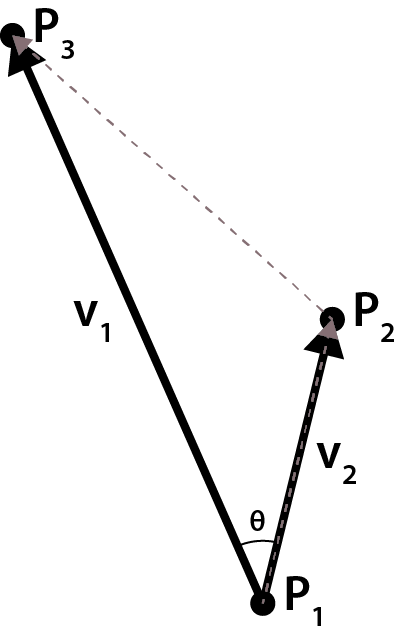
\includegraphics[scale=1]{./img/b_leftRightTurn}
	\caption{The three points $\vec{P_1}$, $\vec{P_2}$ and $\vec{P_3}$. The dashed line represents the path $L$ from points $\vec{P_1}$, through $\vec{P_2}$ to $\vec{P_3}$.}
	\label{fig:b:leftRightTurn}
\end{figure}

Since we are not interested in the exact angle, we only need to know whether $\theta$ is zero and if not what its sign is. To do this we can take the cross-product of the vectors $\vec{v_1}$ and $\vec{v_2}$. The crossproduct of two identical vectors is, no turn, is zero. If the crossproduct is smaller than zero we made a right turn, if it is larger than zero we made a right turn.  

The formal expression, see \autoref{lst:b:formalExpression} for the derivation, is then:
\begin{equation}
	-x_2 y_1 + x_3 y_1 + x_1 y_2 - x_3 y_2 - x_1 y_3 + x_2 y_3.
\end{equation}
Where $x_2$ is the first element of the vector that represents the point $\vec{P_2}$.

\begin{lstlisting}[float, caption={Generation of the formal expression.}, label={lst:b:formalExpression}, language=Mathematica]
p1 = {p1x, p1y, 0};
p2 = {p2x, p2y, 0};
p3 = {p3x, p3y, 0};
v1 = b - a;
v2 = c - a;
Cross[v1, v2]
\end{lstlisting}



